\documentclass[aspectratio=1610,18pt]{ctexbeamer}
\usetheme{Madrid}
% \usefonttheme{professionalfonts}
\usefonttheme{structurebold}
\usecolortheme{rose}
\setbeamerfont{title}{size=\LARGE, series=\bfseries}
\setbeamertemplate{footline}[frame number]



\usepackage{amsmath}
\usepackage{amssymb}
\usepackage{listings}
\usepackage{booktabs}
\usepackage{multirow}
\usepackage{multirow}
\usepackage{lmodern}
\usepackage{xcolor}
\usepackage{float}
\lstset{
  language=Python,  %代码语言使用的是matlab
  % frame=shadowbox, %把代码用带有阴影的框圈起来
  rulesepcolor=\color{red!20!green!20!blue!20},%代码块边框为淡青色
  keywordstyle=\color{blue!90}\bfseries, %代码关键字的颜色为蓝色,粗体
  commentstyle=\color{red!10!green!70}\textit,    % 设置代码注释的颜色
  basicstyle=\footnotesize,
  showstringspaces=true,%不显示代码字符串中间的空格标记
  % numbers=left, % 显示行号
  % numberstyle=8pt,    % 行号字体
  % numberstyle=\color{green},
  stringstyle=\rmfamily\slshape\color[RGB]{128,0,0}, % 代码字符串的特殊格式
  breaklines=true, %对过长的代码自动换行
  extendedchars=false,  %解决代码跨页时,章节标题,页眉等汉字不显示的问题
  escapeinside=``,%代码中出现中文必须加上,否则报错
  texcl=true}

\lstset{breaklines}%自动将长的代码行换行排版

\lstset{extendedchars=false}%解决代码跨页时,章节标题,页眉等汉字不显示的问题

\usepackage{textcomp}
% \usepackage[margin=1in]{geometry}
\usepackage{pythonhighlight}
% \usepackage{minted}
\usepackage[backend=bibtex]{biblatex}
%\usepackage[style=authortitle,backend=biber]{biblatex}
\addbibresource{ResearchRabbit_Export_2022_10_20.bib}

\usepackage{algorithm}
\usepackage{algorithmic}
\renewcommand{\algorithmicrequire}{\textbf{Input:}}
\renewcommand{\algorithmicensure}{\textbf{Output:}}


\title[TDD in quantum]{Reachability Analysis for Quantum Model Checking using TDD}
\subtitle{毕业设计开题报告}
\author{高丁超\\导师:应圣钢}
\usepackage{graphicx}
\usepackage{enumitem}

\setlist[enumerate]{label=\indent\qquad\indent, leftmargin=*,itemsep=30pt}
\setbeamerfont{enumerate item}{size=\LARGE}

\begin{document}

\begin{frame}[plain]
  \titlepage
  \begin{figure}
    \centering
    \begin{minipage}[t]{0.48\textwidth}
    \centering
    
\includegraphics[width=3cm]{iscas.png}
    \end{minipage}
  \end{figure}
\end{frame}
\begin{frame}
  \begin{enumerate}
    \Large
    \item \textbf{Background and significance}
    \item Research of related work
    \item Future work plan
  \end{enumerate}
\end{frame}
% image computation  and quantum basic idea
\begin{frame}
  \begin{align}
    \begin{array}{c}
    {&X=\left[\begin{array}{rr}
    0 & 1 \\
    1 & 0
    \end{array}\right]}&Y=
    {\left[\begin{array}{rr}
    0 & -i \\
    i & 0
    \end{array}\right]}&Z=
    {\left[\begin{array}{rr}
    1 & 0 \\
    0 & -1
    \end{array}\right]} \\
    &H=\frac{1}{\sqrt{2}}\left[\begin{array}{rr}
    1 & 1 \\
    1 & -1
    \end{array}\right]&S=
    {\left[\begin{array}{rr}
    1 & 0 \\
    0 & i
    \end{array}\right]}&T=
    {\left[\begin{array}{lr}
    1 & 0 \\
    0 & e^{i \pi / 4}
    \end{array}\right]}
    \end{array}\\
    \left[\begin{array}{llll}
    1 & 0 & 0 & 0 \\
    0 & 1 & 0 & 0 \\
    0 & 0 & 0 & 1 \\
    0 & 0 & 1 & 0
    \end{array}\right]\\
    \left[\begin{array}{rrrr}
    1 & 0 & 0 & 0 \\
    0 & 1 & 0 & 0 \\
    0 & 0 & 1 & 0 \\
    0 & 0 & 0 & -1
    \end{array}\right]\\
    \left[\begin{array}{llll}
    1 & 0 & 0 & 0 \\
    0 & 0 & 1 & 0 \\
    0 & 1 & 0 & 0 \\
    0 & 0 & 0 & 1
    \end{array}\right]
    \end{align}
\end{frame}
\begin{frame}
  \begin{enumerate}
    \Large
    \item  transition system: $(S, I, \Sigma, T)$
    \begin{equation}
      where
      \begin{cases}
        x = x_1, \cdots, x_n\\
        y = y_1, \cdots, y_n\\
        \sigma = \sigma_1, \cdots, \sigma_m
      \end{cases}
      \notag
    \end{equation}
    \item Quantum transition system: $(S, S_0, \Sigma, R)$
  \end{enumerate}
\end{frame}
\begin{frame}
  \begin{figure}
    \centering
    \begin{minipage}[t]{0.48\textwidth}
    \centering
    \scalebox{0.8}{
    \begin{quantikz}[column sep=0.28cm,row sep=0.15cm]%
                  &\ctrl{3}&\qw     &\ctrl{5}&\qw     &\qw     &\qw     &\qw     &\gate{X}&\qw&\qw&\qw \\
                  &\qw     &\ctrl{2}&\qw     &\ctrl{3}&\qw     &\qw     &\qw     &\qw&\gate{X}&\qw&\qw \\
                  &\qw     &\qw     &\qw     &\qw     &\ctrl{2}&\ctrl{3}&\qw     &\qw&\qw&\gate{X}&\qw \\
\lstick{$\ket{0}$}&\gate{X}&\gate{X}&\qw     &\qw     &\qw     &\qw     &\meter{}&\cwbend{-3}&\cwbend{-2} \\
\lstick{$\ket{0}$}&\qw     &\qw     &\qw     &\gate{X}&\gate{X}&\qw     &\meter{}&\cw&\cwbend{-1}&\cwbend{-2} \\
\lstick{$\ket{0}$}&\qw     &\qw     &\gate{X}&\qw     &\qw     &\gate{X}&\meter{}&\cwbend{-2}&\cw&\cwbend{-1}
    \end{quantikz}
    }
    \end{minipage}
    \begin{minipage}[t]{0.48\textwidth}
    \centering
    $\text { CNOT }=\left[\begin{array}{llll}
      1 & 0 & 0 & 0 \\
      0 & 1 & 0 & 0 \\
      0 & 0 & 0 & 1 \\
      0 & 0 & 1 & 0
      \end{array}\right]$
    \end{minipage}
  \end{figure}
\end{frame}
% TDD
% results
\begin{frame}
  \begin{figure}
    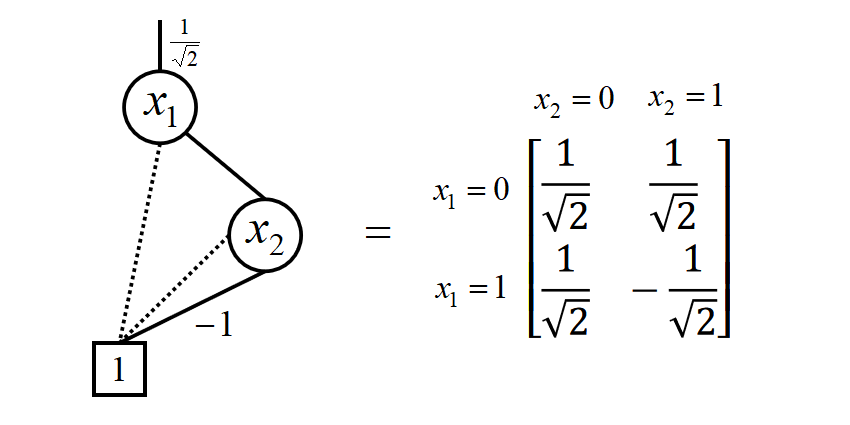
\includegraphics[width = .8\textwidth]{TDD_H_gate2.png}
  \end{figure}
\end{frame}
\begin{frame}
  \begin{figure}[tbh]
      \centering
      \scalebox{0.8}{
      \begin{minipage}{0.3\textwidth}
      \small
    \[P=\frac{1}{6}\begin{bmatrix}
    1&-1  &1&-1  & 1&-1 &0&0\\
    -1&1  &-1&1  & -1&1 &0&0\\
    1&-1  &1&-1  & 1&-1 &0&0\\
    -1&1  &-1&1  & -1&1 &0&0\\
    1&-1  &1&-1  & 1&-1 &0&0\\
    -1&1  &-1&1  & -1&1 &0&0\\
    0&0   &0&0   &0&0   &3&-3\\
    0&0   &0&0   &0&0   &-3&3\\
    \end{bmatrix}
    \]
      \end{minipage}
     }
     \quad
     \hfil
      \begin{minipage}{0.5\textwidth}  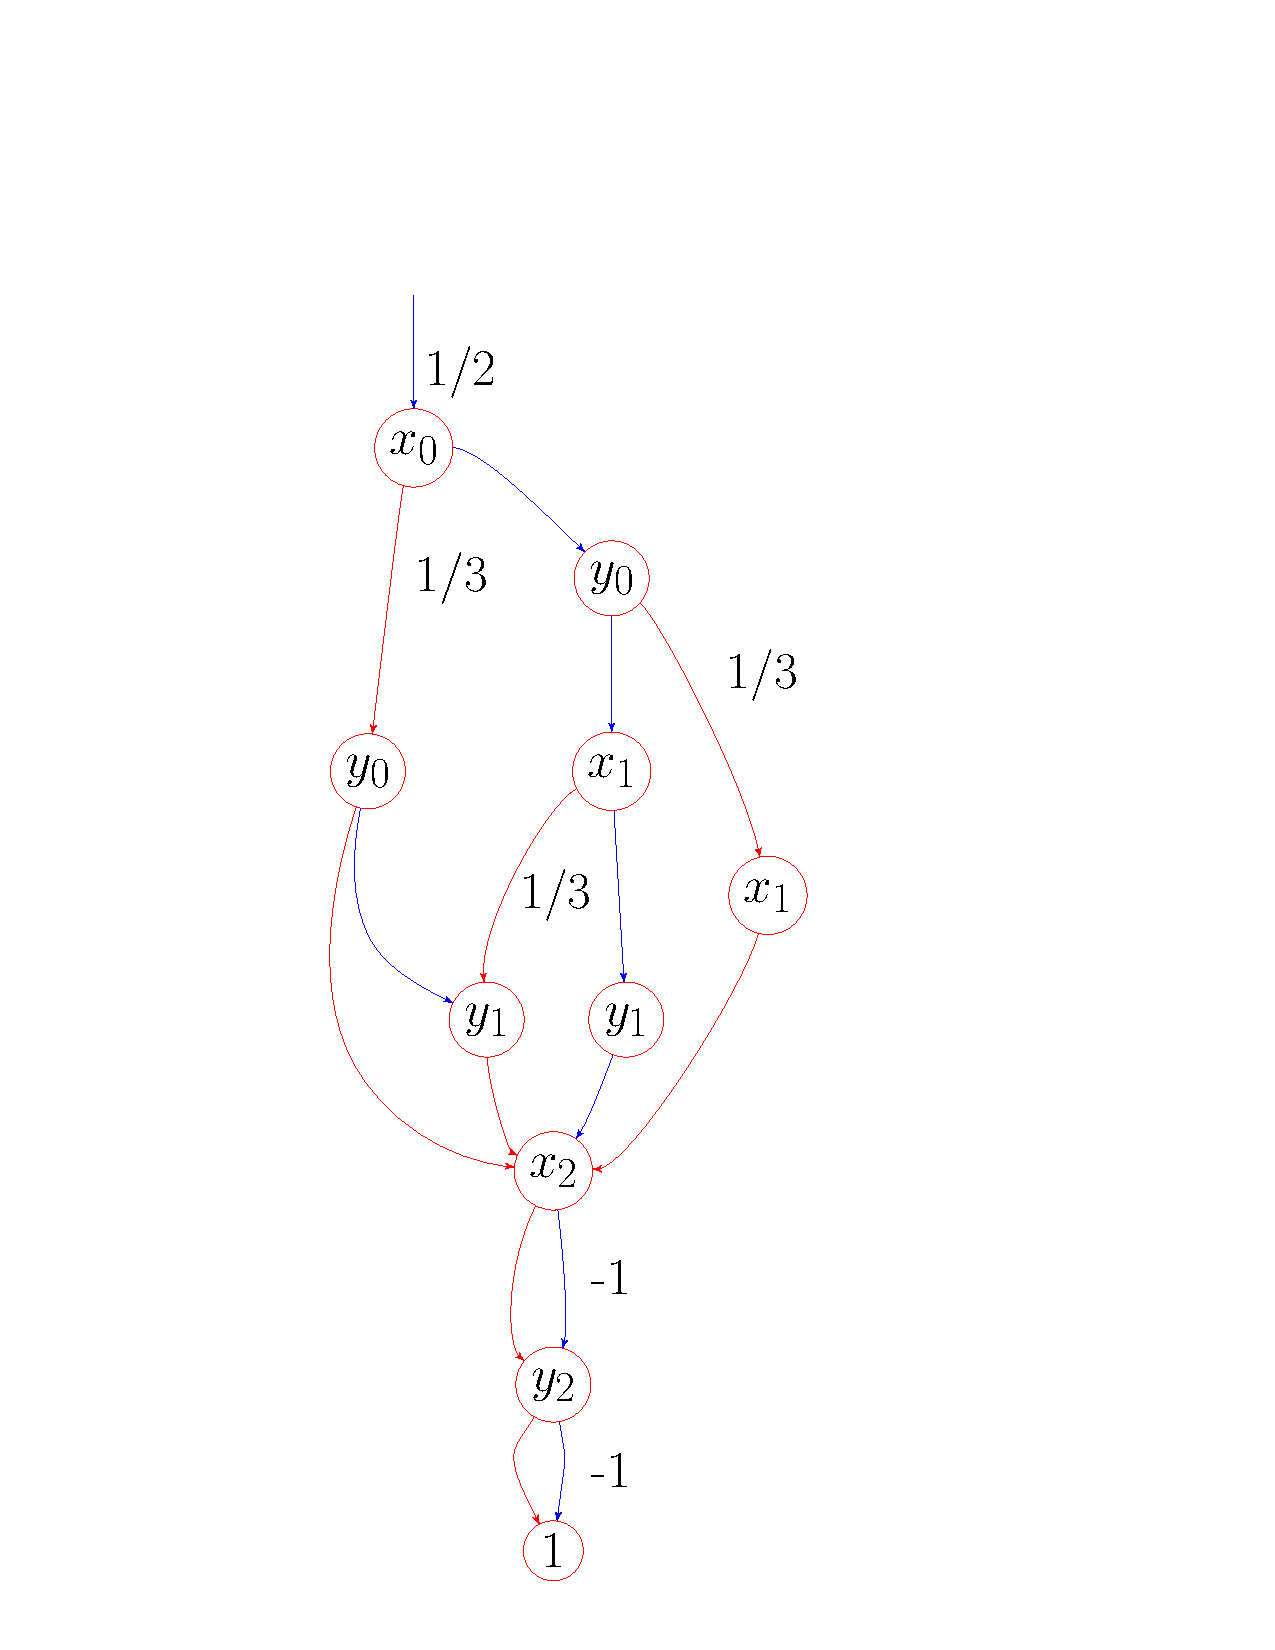
\includegraphics[width=\textwidth]{Projector.pdf}
      \end{minipage}
    \end{figure}
\end{frame}
\begin{frame}
  \begin{table}[]
    \Large
    \rule{0pt}{30pt}
    \begin{tabular}{l|c}
    benchmark & time \\\hline
    Grover 20       & $\sim$5min  \\
    Quantum Fourier Transform 20           & $\sim$20min \\
    Quantum Random walk 20           & $\sim$6min\\
    Bernstein-Vazirani 50           & $\sim$4min  \\
    GHZ 500         & $\sim$3sec \\
    \end{tabular}
    \end{table}
\end{frame}
\begin{frame}
  \begin{figure}[h]
    \centering
    \scalebox{1}{
    \begin{tikzpicture}
 
    \node at (0,0) [anchor=north]{
    \begin{quantikz}[column sep=0.28cm,row sep=0.6cm]
    &\ctrl{1}&\gate{H}&\qw&\gate{X}&\qw&\qw&\qw     &\ctrl{1}&\qw&\qw&\qw     &\gate{X}&\qw&\gate{H}&\qw \\
    &\ctrl{1}&\gate{H}&\qw&\gate{X}&\qw&\gate{H}&\qw&\gate{X}&\qw&\gate{H}&\qw&\gate{X}&\qw&\gate{H}&\qw \\
    &\gate{X}&\qw     &\qw     &\qw     &\qw     &\qw     &\qw     &\qw     &\qw&\qw&\qw&\qw&\qw&\qw&\qw&\qw 
    \end{quantikz}};
    \end{tikzpicture}
    }
    \end{figure}
\end{frame}
\begin{frame}
  \begin{figure}
    \centering
    \scalebox{1}{
    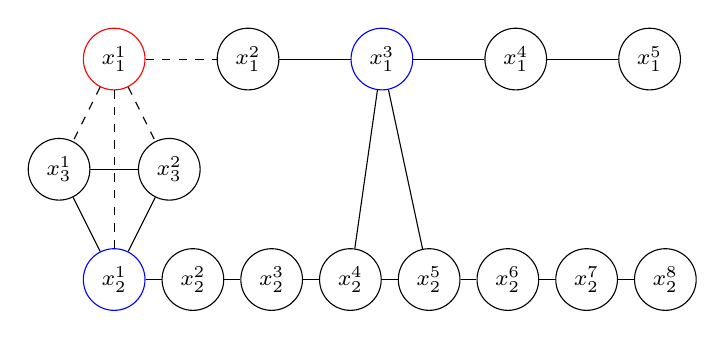
\begin{tikzpicture}
\node[circle, minimum width =10pt , minimum height =10pt ,draw= red] (1) at(0,2){\begin{footnotesize}$x_1^1$\end{footnotesize}};
\node[circle, minimum width =10pt , minimum height =10pt ,draw=black] (2) at(1.7,2){\begin{footnotesize}$x_1^2$\end{footnotesize}};
\node[circle, minimum width =10pt , minimum height =10pt ,draw=blue] (3) at(3.4,2){\begin{footnotesize}$x_1^3$\end{footnotesize}};
\node[circle, minimum width =10pt , minimum height =10pt ,draw=black] (4) at(5.1,2){\begin{footnotesize}$x_1^4$\end{footnotesize}};
\node[circle, minimum width =10pt , minimum height =10pt ,draw=black] (5) at(6.8,2){\begin{footnotesize}$x_1^5$\end{footnotesize}};
\node[circle, minimum width =10pt , minimum height =10pt ,draw=black] (6) at(-0.7,0.6){\begin{footnotesize}$x_3^1$\end{footnotesize}};
\node[circle, minimum width =10pt , minimum height =10pt ,draw=black] (7) at(0.7,0.6){\begin{footnotesize}$x_3^2$\end{footnotesize}};
\node[circle, minimum width =10pt , minimum height =10pt ,draw=blue] (8) at(0,-0.8){\begin{footnotesize}$x_2^1$\end{footnotesize}};
\node[circle, minimum width =10pt , minimum height =10pt ,draw=black] (9) at(1,-0.8){\begin{footnotesize}$x_2^2$\end{footnotesize}};
\node[circle, minimum width =10pt , minimum height =10pt ,draw=black] (10) at(2,-0.8){\begin{footnotesize}$x_2^3$\end{footnotesize}};
\node[circle, minimum width =10pt , minimum height =10pt ,draw=black] (11) at(3,-0.8){\begin{footnotesize}$x_2^4$\end{footnotesize}};
\node[circle, minimum width =10pt , minimum height =10pt ,draw=black] (12) at(4,-0.8){\begin{footnotesize}$x_2^5$\end{footnotesize}};
\node[circle, minimum width =10pt , minimum height =10pt ,draw=black] (13) at(5,-0.8){\begin{footnotesize}$x_2^6$\end{footnotesize}};
\node[circle, minimum width =10pt , minimum height =10pt ,draw=black] (14) at(6,-0.8){\begin{footnotesize}$x_2^7$\end{footnotesize}};
\node[circle, minimum width =10pt , minimum height =10pt ,draw=black] (15) at(7,-0.8){\begin{footnotesize}$x_2^8$\end{footnotesize}};
\draw[dashed] (1) --(2);
\draw[-] (2)--(3) --(4)--(5);
\draw[-] (6)--(7);
\draw[-] (8)--(9)--(10)--(11)--(12)--(13)--(14)--(15);
\draw[dashed] (1)--(6)  (1)--(7);
\draw[-] (8)--(6)  (8)--(7);
\draw[-] (3)--(11)  (3)--(12);
\draw[dashed] (1)--(8);

\end{tikzpicture}
}
\end{figure}
\end{frame}

\begin{frame}
  \begin{figure}
    \centering
    \scalebox{1}{
    \begin{tikzpicture}
    % \draw[dotted, red, line width =1.5pt] (-4.05,-0.3) rectangle (-2.35,-3.05);
    % \draw[dotted, blue, line width =1.5pt] (-2.24,-0.3) -- (-2.24,-4.6) -- (1.15,-4.6)--(1.15,-1.6)--(0.45,-1.6)--(0.45,-3.9)--(-1.54,-3.9)--(-1.54,-0.3)--(-2.24,-0.3);
    % \draw[dotted, green, line width =1.5pt] (-1.4,-1) rectangle (0.3,-3.8);
    \draw[dotted, red, line width =2pt] (-4.3,-2.15) -- (2.4,-2.15);
    \draw[dotted, blue, line width =1.8pt] (-2.3,0) -- (-2.3,-4.7);
    \draw[dotted, blue, line width =1.8pt] (-0.55,0) -- (-0.55,-4.7);
    \node at (0,0) [anchor=north]{
    \begin{quantikz}[column sep=0.28cm,row sep=0.15cm]%
                  &\ctrl{3}&\qw     &\ctrl{5}&\qw     &\qw     &\qw     &\qw     &\gate{X}&\qw&\qw&\qw \\
                  &\qw     &\ctrl{2}&\qw     &\ctrl{3}&\qw     &\qw     &\qw     &\qw&\gate{X}&\qw&\qw \\
                  &\qw     &\qw     &\qw     &\qw     &\ctrl{2}&\ctrl{3}&\qw     &\qw&\qw&\gate{X}&\qw \\
\lstick{$\ket{0}$}&\gate{X}&\gate{X}&\qw     &\qw     &\qw     &\qw     &\meter{}&\cwbend{-3}&\cwbend{-2} \\
\lstick{$\ket{0}$}&\qw     &\qw     &\qw     &\gate{X}&\gate{X}&\qw     &\meter{}&\cw&\cwbend{-1}&\cwbend{-2} \\
\lstick{$\ket{0}$}&\qw     &\qw     &\gate{X}&\qw     &\qw     &\gate{X}&\meter{}&\cwbend{-2}&\cw&\cwbend{-1}
    \end{quantikz}
    };
    \end{tikzpicture}}
\end{figure}
\end{frame}
\begin{frame}
  \begin{table}[]
    \Large
    \rule{0pt}{30pt}
    \begin{tabular}{l|ccc}
    benchmark & basic & addition& contraction \\\hline
    Grover 20       & $\sim$5min  & $\sim$4min & $\sim$4sec  \\
    Quantum Fourier Transform 20           & $\sim$20min & $\sim$11min & $<$1sec \\
    Quantum Random walk 20           & $\sim$6min & $\sim$4min & $\sim$15sec\\
    Bernstein-Vazirani 50           & $\sim$4min & $\sim$4min & $\sim$16sec \\
    GHZ 500         & $\sim$3sec & $\sim$1.5sec & $\sim$1.7sec\\
    \end{tabular}
    \end{table}
\end{frame}
\begin{frame}
  \begin{table}[]
    \centering
    \Large
    \scalebox{1}{
    \begin{tabular}{c|cccc}
                         circuit  & & $k=0$ & $k=1$ & $k=3$ \\\hline
    \multirow{2}{*}{Grover\_40}    &time       & 1,510.42   &1,519.24 & 1,495.20  \\
                            &max \#node     &589,865     & 393,423 & 245,814  \\\hline
    \multirow{2}{*}{QFT\_100}   &time       &121.28    & 118.78 & 128.31\\
                                 & max \#node     &524,369     & 262,226 & 131,155\\
    \end{tabular}
    }
    \end{table}
\end{frame}
\begin{frame}
  \begin{enumerate}
    \Large
    \item efficient quantum image computation algorithms
    \item contraction partition-based algorithm
  \end{enumerate}
\end{frame}
\end{document}